\documentclass{article}
\usepackage[utf8]{inputenc}
\usepackage{multicol}
\usepackage{listings}
\usepackage{verbatim}
\usepackage{color}
\usepackage{geometry}

\usepackage{float}
\usepackage{amsmath}
\usepackage{hyperref}
\setlength{\belowcaptionskip}{-10pt}
\setlength{\abovecaptionskip}{-30pt}
\floatstyle{boxed} 
\restylefloat{figure}
\usepackage{graphicx}
\definecolor{codegreen}{rgb}{0,0.6,0}
\definecolor{codegray}{rgb}{0.5,0.5,0.5}
\definecolor{codepurple}{rgb}{0.58,0,0.82}
\definecolor{backcolour}{rgb}{0.95,0.95,0.92}

\lstdefinestyle{mystyle}{
	backgroundcolor=\color{backcolour},   
	commentstyle=\color{codegreen},
	keywordstyle=\color{blue},
	numberstyle=\tiny\color{codegray},
	stringstyle=\color{codepurple},
	basicstyle=\footnotesize,
	breakatwhitespace=false,         
	breaklines=true,                 
	captionpos=b,                    
	keepspaces=true,                 
	numbers=left,                    
	numbersep=5pt,                  
	showspaces=false,                
	showstringspaces=false,
	showtabs=false,                  
	tabsize=2
}

\lstset{style=mystyle}
\title{Data Mining\\
		Home work 04\\Descriptive Statistics}
<<<<<<< HEAD
\author{Aqeel Labash\\ \textbf{Lecturer:} Jaak Vilo}
\date{6 March 2016}
=======
\author{Aqeel Labash\\ \textbf{Supervisor:} Jaak Vilo}
\date{17 February 2016}
>>>>>>> 59314da8caff27eef4431dda7d1964df874949c5
\geometry{
	a4paper,
	total={170mm,257mm},
	left=10mm,
	top=5mm,
}
\begin{document}
	\maketitle
	\section*{First Question}
	The things that I took home is :) :
	\begin{enumerate}
\item  Each data type has it's own
\item When we want to compare data to each other it's always better for the plot of the groups to be more scalable for people eyes.
\item If we are using line width to show information , there should be a fixed max width.
\item When using color for categories, the max number we should use is 6-12 color , otherwise the reader will get lost between the color's.
\item It's better to use separable channels for different abstract dimensions.
\item There is no bad or good way to show data, but it should match our goal.
\item Using 3d visualization should be accompanied with extra caution.Because what we think it's more clear may delay the information delivery.
\item In 3d visualization the depth take away ability of comparison because of perspective distortion.
\item When we have complex changes it's better to use series of visualization rather than animation because we lose track of global changes and focus on local changes.
\item Validate against the right threat.
	\end{enumerate}
	\section*{Second Question}
While trying to plot I found an outliers or damaged data (height , weight less than zero ) there was about 3472 row. I cleaned them using the following code:
\begin{lstlisting}[language=R]
#### Second Question ######
ncmp = read.csv('ncmp_1415_final_non_disclosive.csv',header = TRUE)
nrow(ncmp[ncmp$height<0,])
ncmp <- ncmp[ncmp$height>0,]
\end{lstlisting}
\textbf{Note:}The data later changed on the homework page with clean data, anyway I sticked to this data since I already started with it.
In the following figure I plotted the requested combination (age,height,bmi,age) while showing the gender in colors.
\begin{figure}[H]
\begin{center}
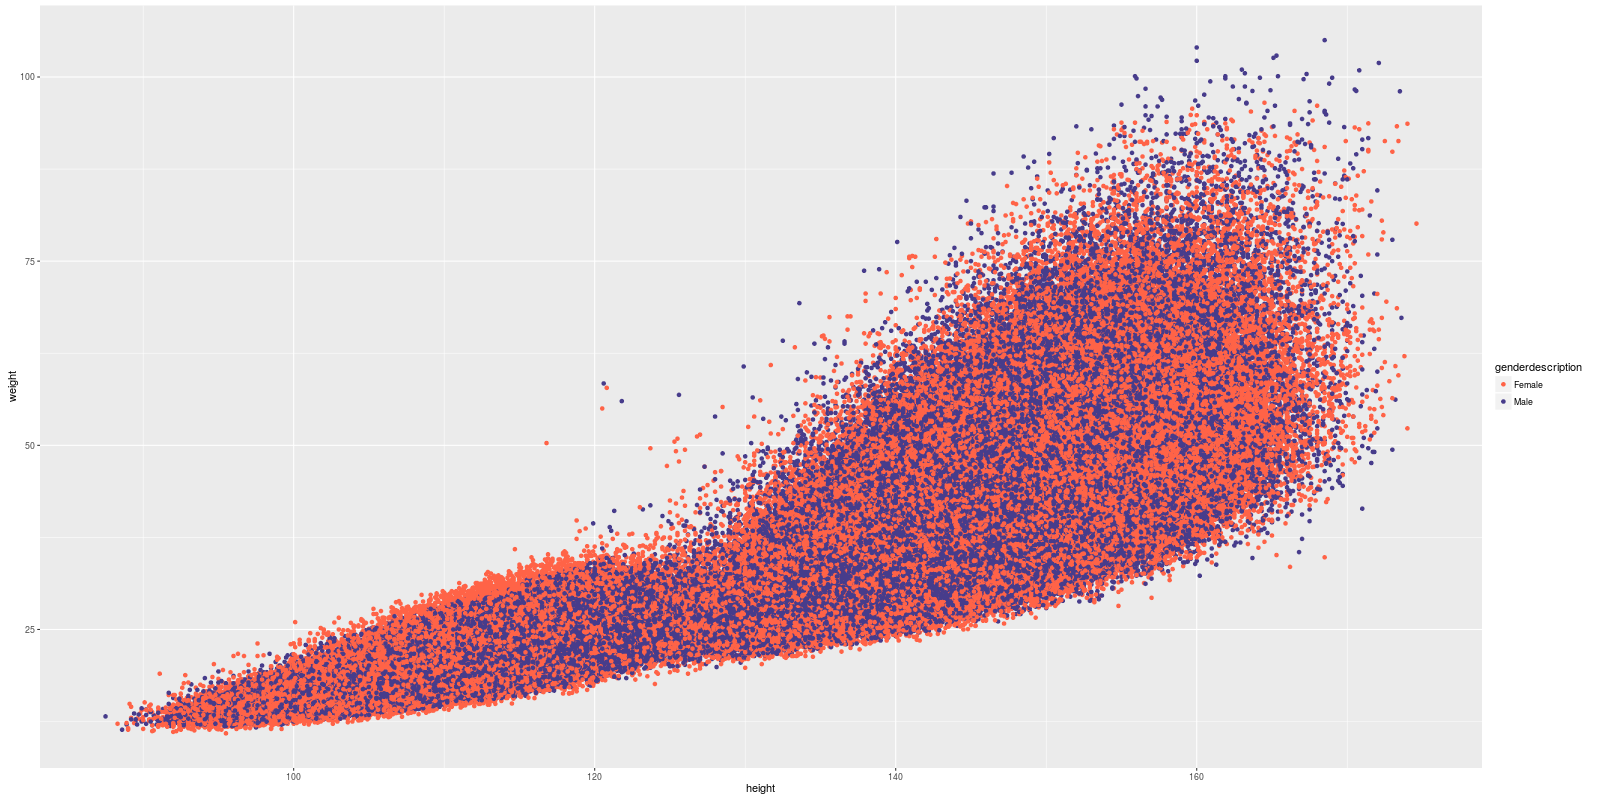
\includegraphics[scale=0.3]{heightweightgender.png}
\end{center}
\caption{Height vs weight}
\end{figure}
In the previous plot we notice the increase of height lead to increase of weight as well.
\begin{figure}[H]
	\begin{center}
		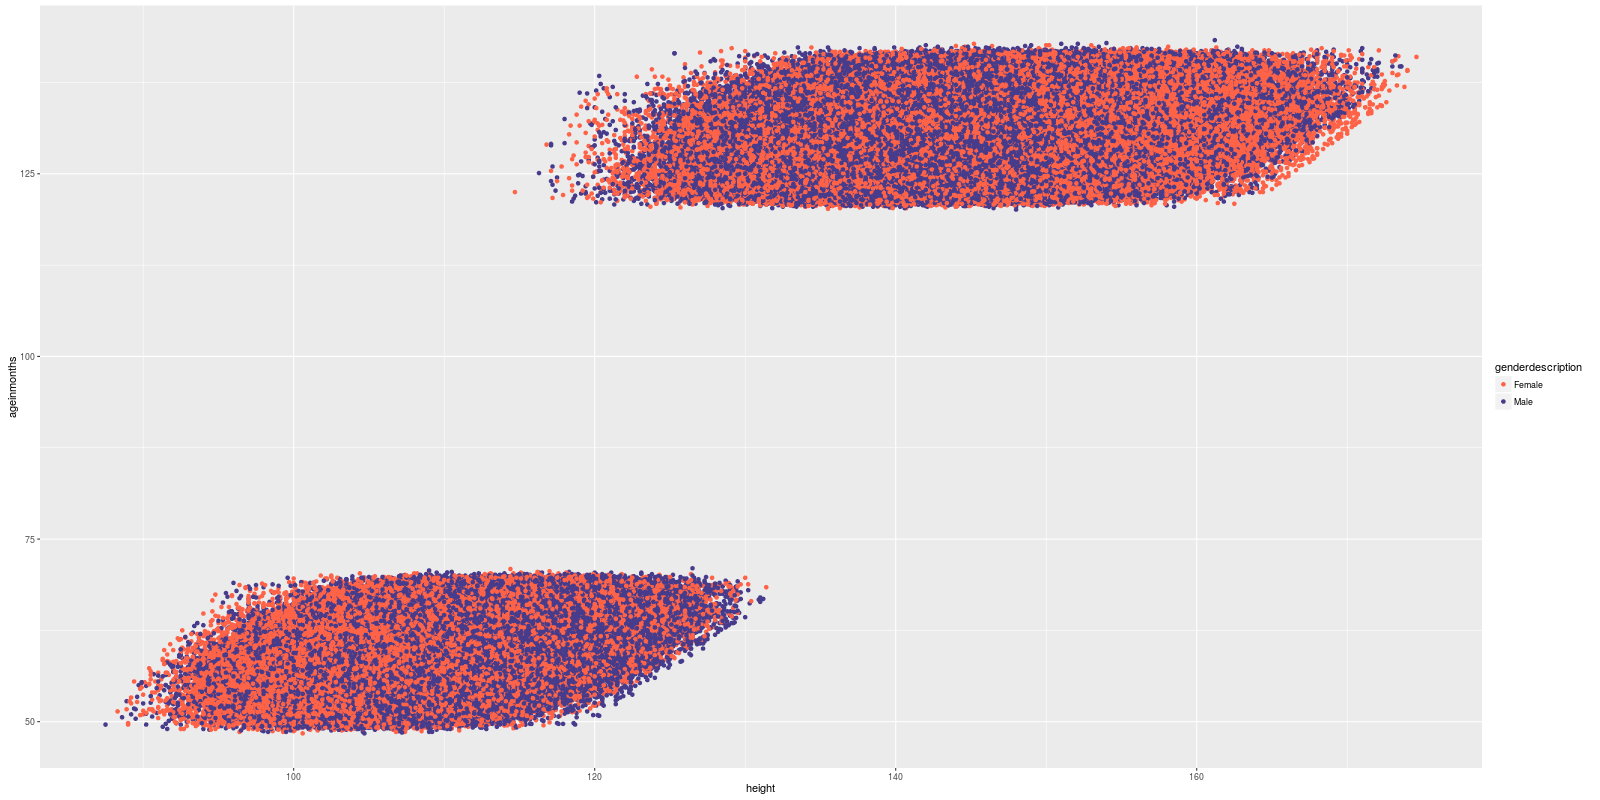
\includegraphics[scale=0.3]{heightage.png}
	\end{center}
	\caption{Height vs Age}
\end{figure}
	In this figure we notice that there is a break in the data which cause this empty area.
\begin{figure}[H]
	\begin{center}
		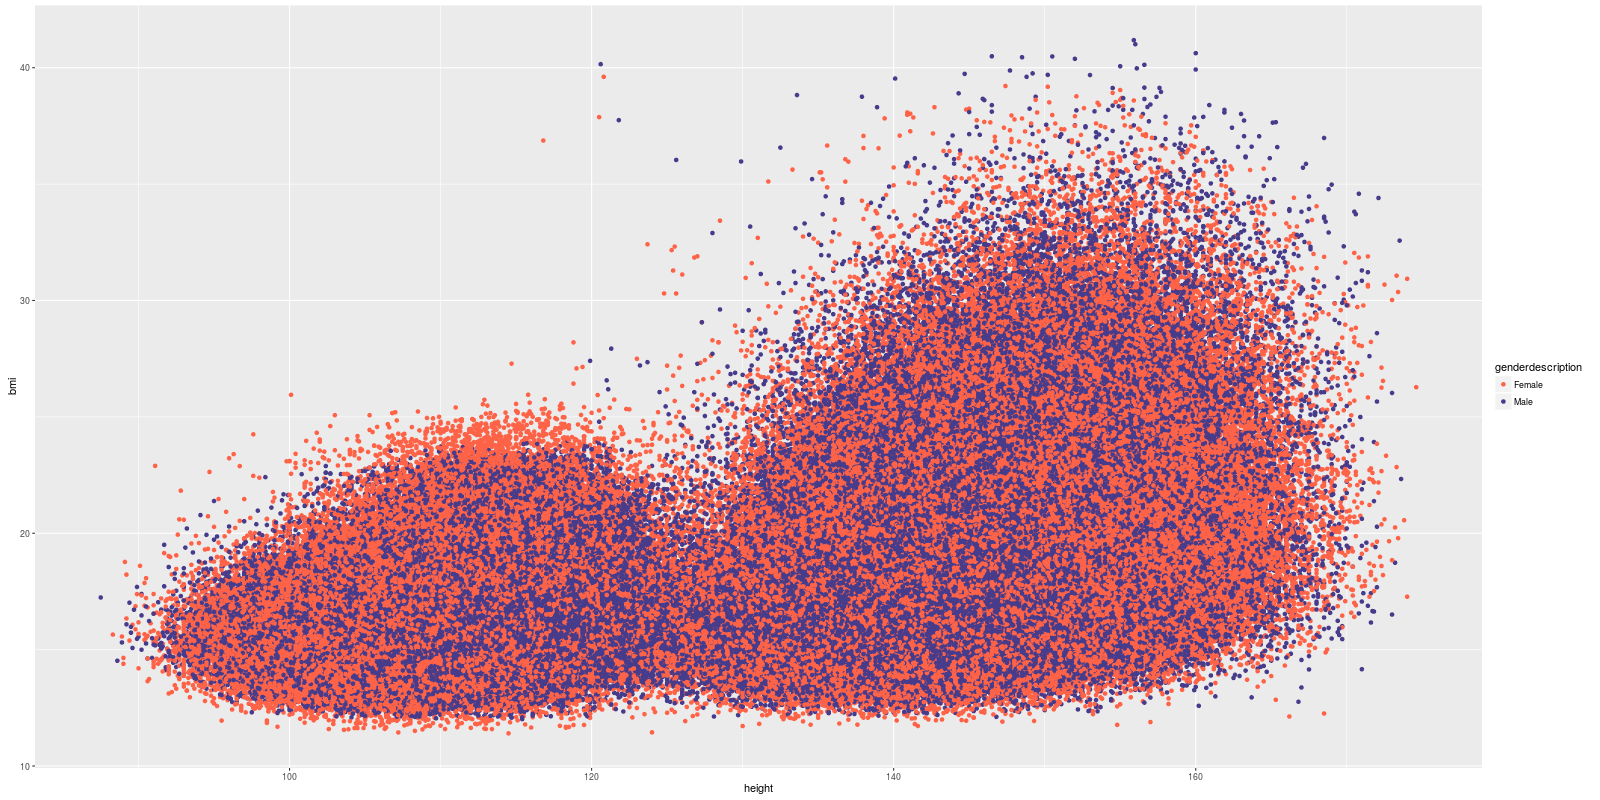
\includegraphics[scale=0.3]{heightBMI.png}
	\end{center}
	\caption{Height vs BMI}
\end{figure}
In the previous figure we notice the higher the higher BMI.
\begin{figure}[H]
	\begin{center}
		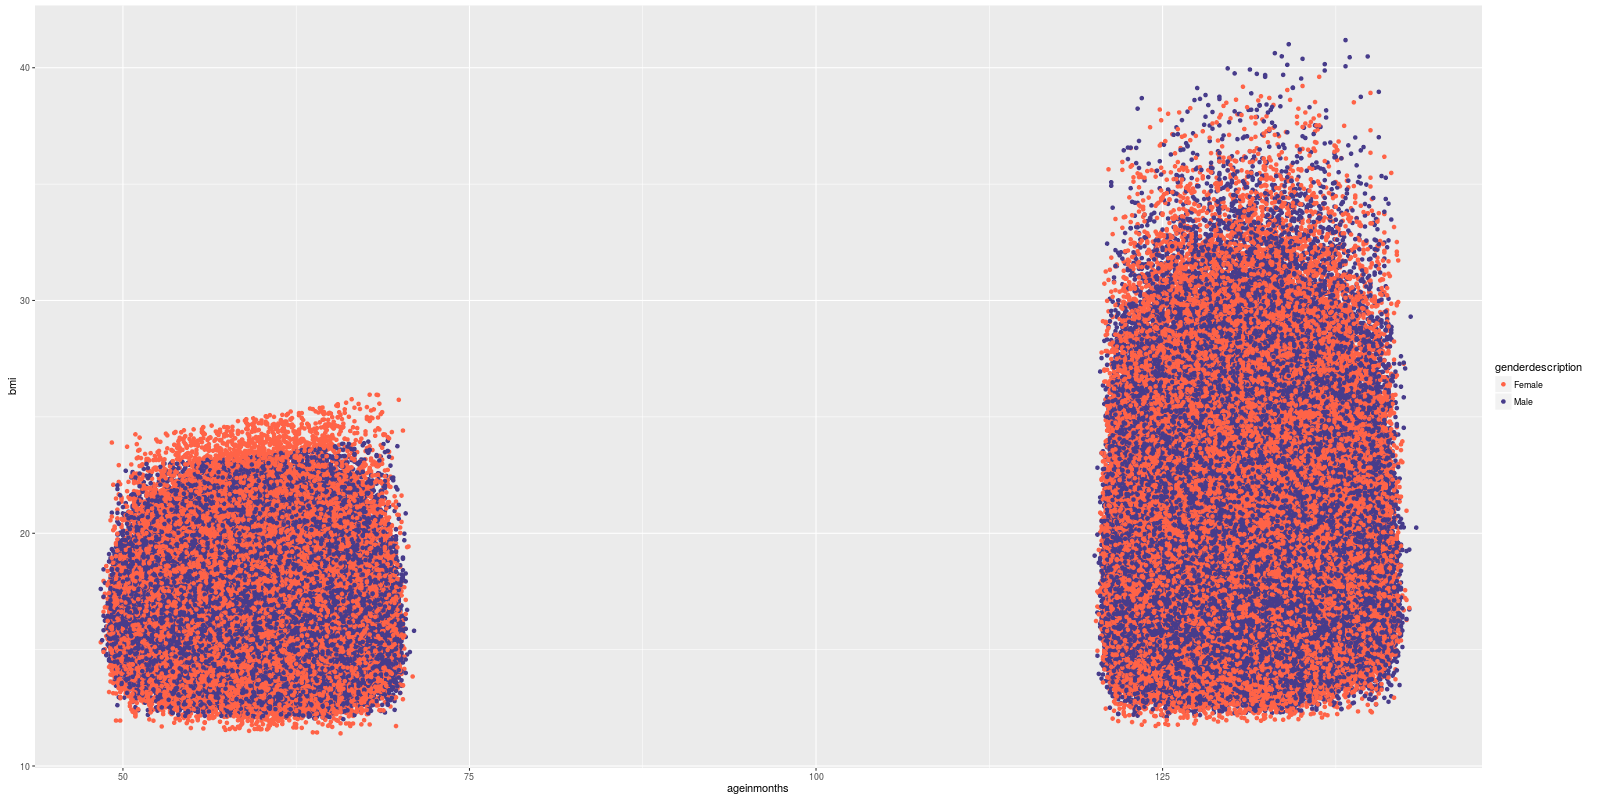
\includegraphics[scale=0.3]{ageBMI.png}
	\end{center}
	\caption{Age vs BMI}
\end{figure}
In Figure 4 we can see that we have two quantiles of ages. And the older the more BMI.
\begin{figure}[H]
	\begin{center}
		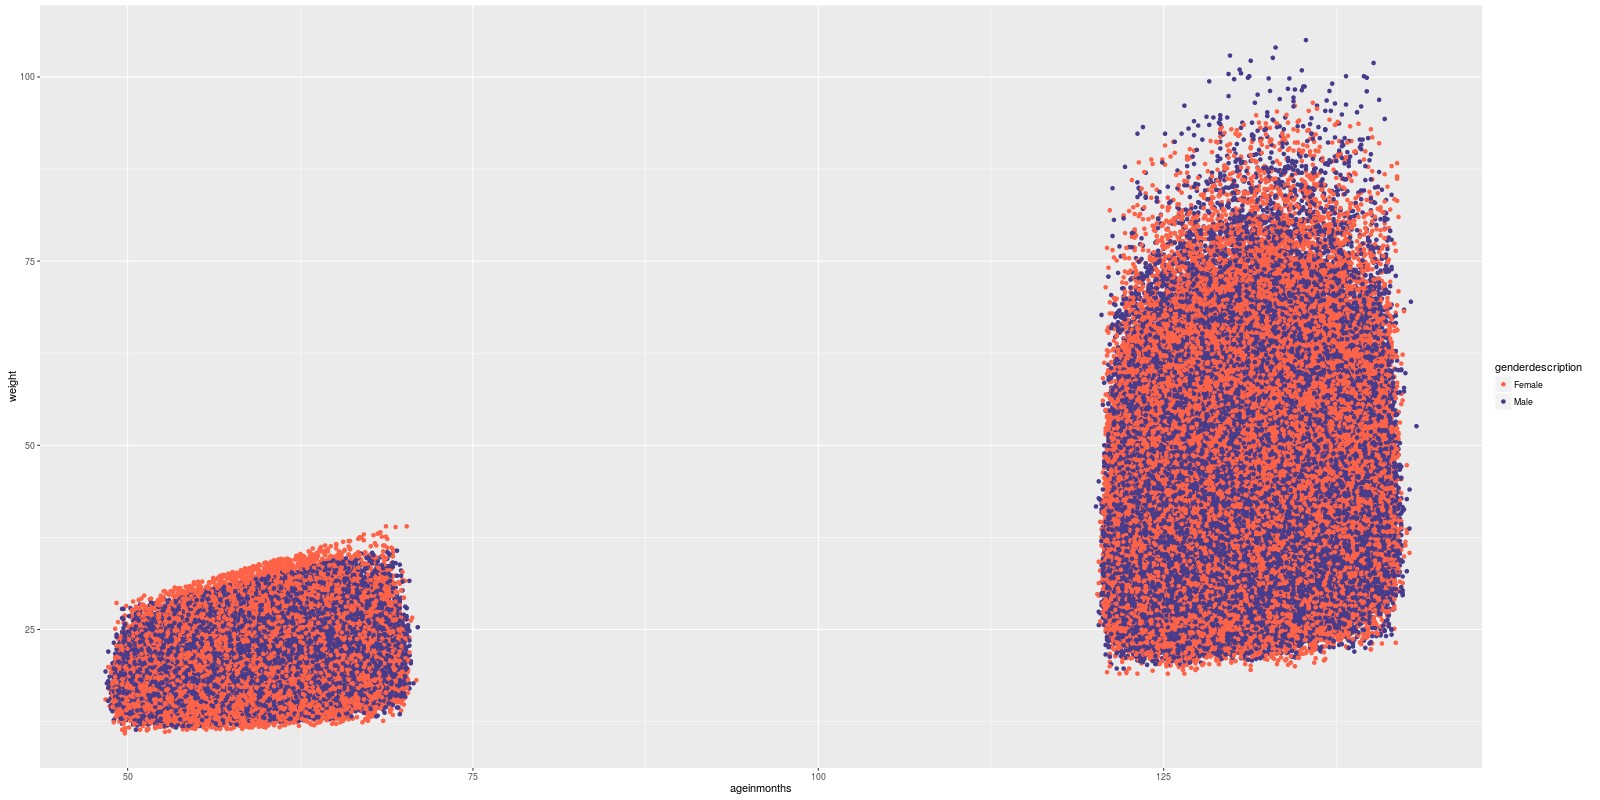
\includegraphics[scale=0.3]{ageweight.png}
	\end{center}
	\caption{Age vs weight}
\end{figure}
It's expected here where the age increase , the weight increase as well.
\begin{figure}[H]
	\begin{center}
		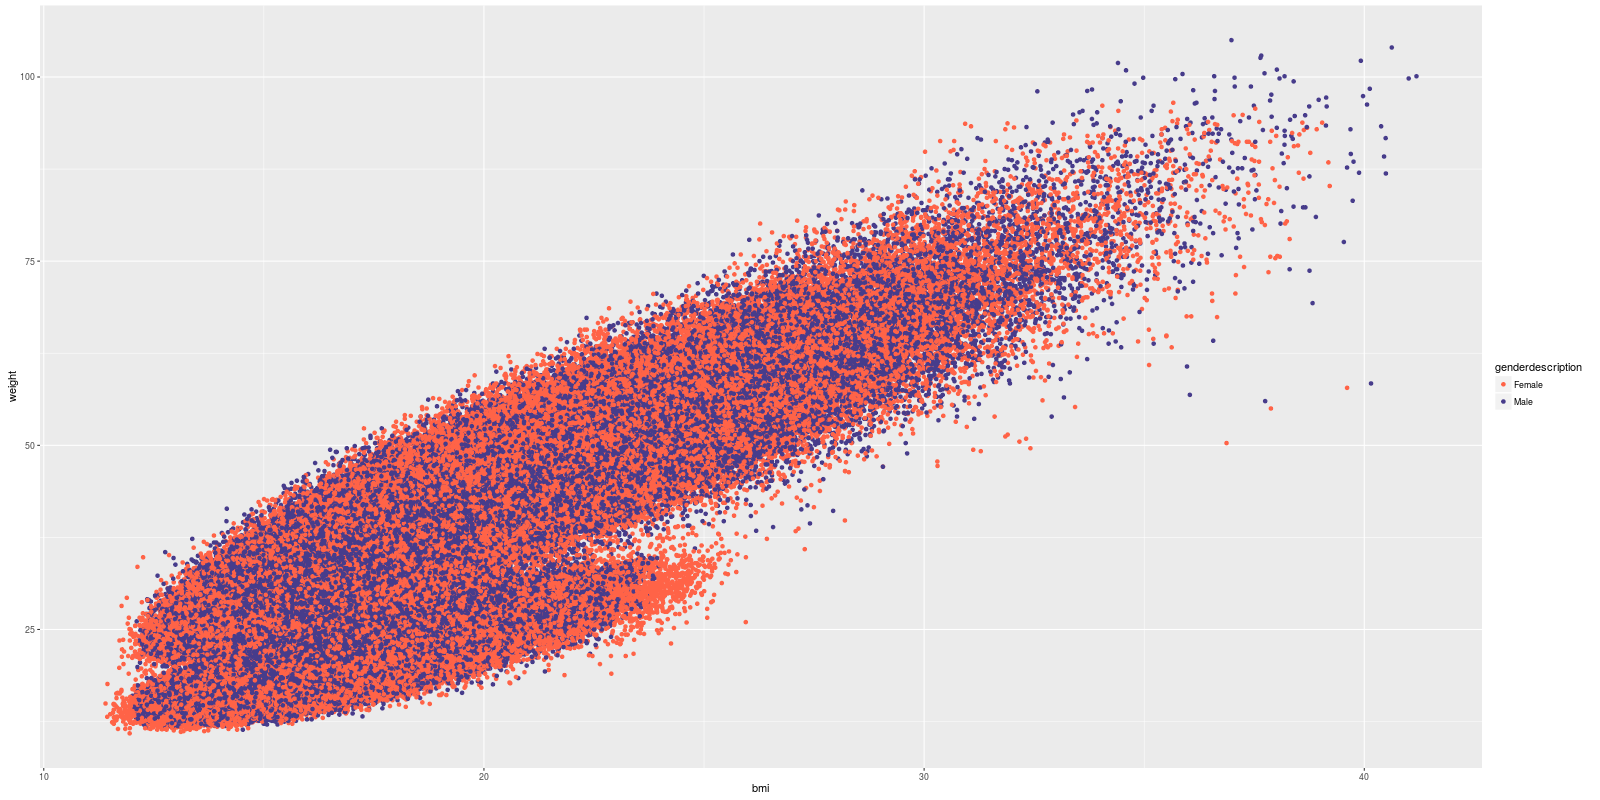
\includegraphics[scale=0.3]{BMIweight.png}
	\end{center}
	\caption{BMI vs weight}
\end{figure}
In figure 6 we can see that increasing in weight mean increase in BMI.
<<<<<<< HEAD
\(BMI = \frac{weight}{height^2}\) \\
=======
\(BMI = \frac{weight}{height^2}\)
>>>>>>> 59314da8caff27eef4431dda7d1964df874949c5
\textbf{Note:}Although the previous plots looks cool (for me at least :) ) but I think there isn't much information we can get from.
To plot the previous figures I used the following code:
\begin{lstlisting}[language=R]
library(ggplot2)
#Height Weight
png('heightweight.png',height = 800,width = 1600)
qplot(height,weight,colour =genderdescription,data = ncmp)+ 
scale_color_manual(values=c("tomato", "slateblue4"))
dev.off()
# Height Age
png('heightage',height = 800,width = 1600)
qplot(height,ageinmonths,colour =genderdescription,data = ncmp)+ 
scale_color_manual(values=c("tomato", "slateblue4"))
dev.off()
# Height BMI
png('heightBMI',height = 800,width = 1600)
qplot(height,bmi,colour =genderdescription,data = ncmp)+ 
scale_color_manual(values=c("tomato", "slateblue4"))
dev.off()
# age BMI
png('ageBMI',height = 800,width = 1600)
qplot(ageinmonths,bmi,colour =genderdescription,data = ncmp)+ 
scale_color_manual(values=c("tomato", "slateblue4"))
dev.off()

# age weight
png('ageweight',height = 800,width = 1600)
qplot(ageinmonths,weight,colour =genderdescription,data = ncmp)+ 
scale_color_manual(values=c("tomato", "slateblue4"))
dev.off()

# BMI weight
png('BMIweight',height = 800,width = 1600)
qplot(bmi,weight,colour =genderdescription,data = ncmp)+ 
scale_color_manual(values=c("tomato", "slateblue4"))
dev.off()

\end{lstlisting}
In the following figure we can see the caterogical bmi of the kids depending on there age,and BMI : 
\begin{figure}[H]
	\begin{center}
		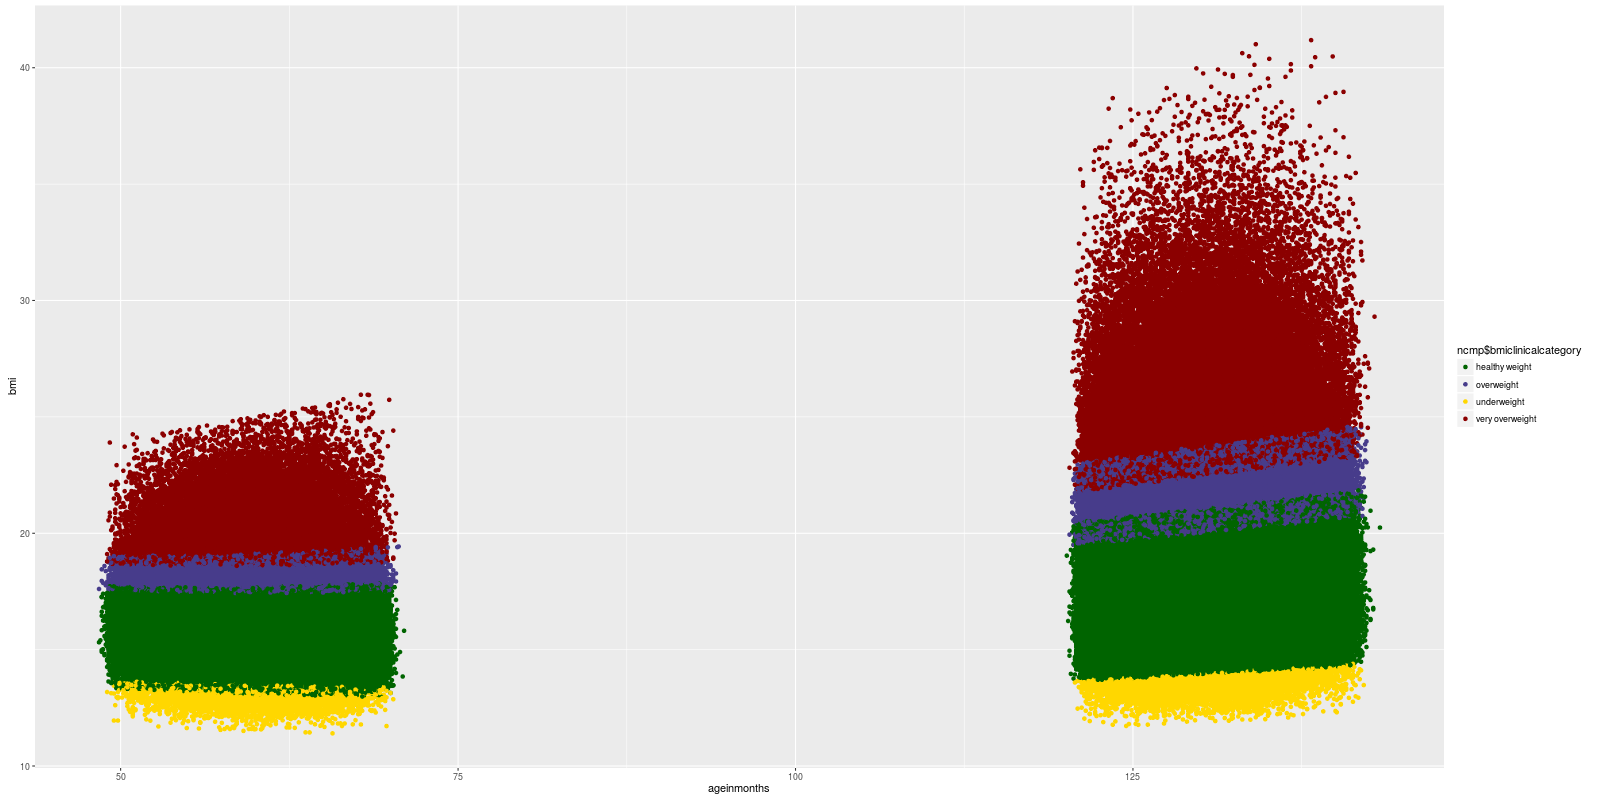
\includegraphics[scale=0.3]{bmicatage.PNG}
	\end{center}
	\caption{age vs BMI}
\end{figure}
And here is the code that generated the previous figure.
\begin{lstlisting}[language=R]
#bmi category with age
png('bmicatage',height = 800,width = 1600)
qplot(ageinmonths,bmi,colour =ncmp$bmiclinicalcategory,data = ncmp)+
scale_color_manual(values=c("darkgreen", "slateblue4","gold","darkred"))
dev.off()
\end{lstlisting}
	\section*{Third Question}
	For this question I used Mosteller formula to calculate Body Surface Area \(BSA =\frac{\sqrt{W\times H}}{60}\)
<<<<<<< HEAD
	In the following plots I colored them depending to BMI clinical category because it was continuous at some ranges. And BMI linked to weight and height.\\ \textbf{Note:}All images (colored by gender or BMI categorical) can be seen at full resolution \href{https://github.com/aqeel13932/DM/tree/master/HW04}{here}
=======
	In the following plots I colored them depending to BMI clinical category because it was continuous at some ranges. 
>>>>>>> 59314da8caff27eef4431dda7d1964df874949c5
	\begin{figure}[H]
		\begin{center}
			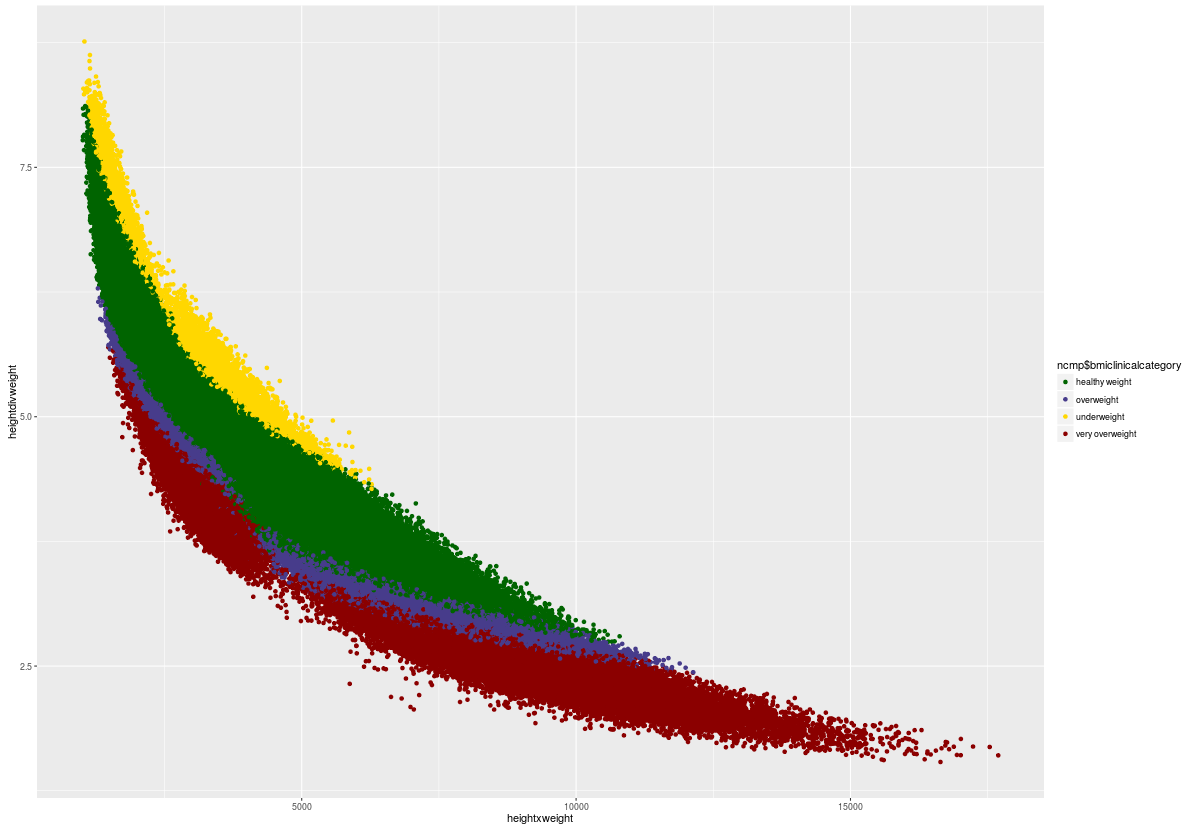
\includegraphics[scale=0.4]{xdiv.png}
		\end{center}
		\caption{Multiplication vs Devision of height and weight }
	\end{figure}
<<<<<<< HEAD
	In figure 8 we can see how BMI category can be contaminated by rule between height and weight.
=======
	
>>>>>>> 59314da8caff27eef4431dda7d1964df874949c5
		\begin{figure}[H]
			\begin{center}
				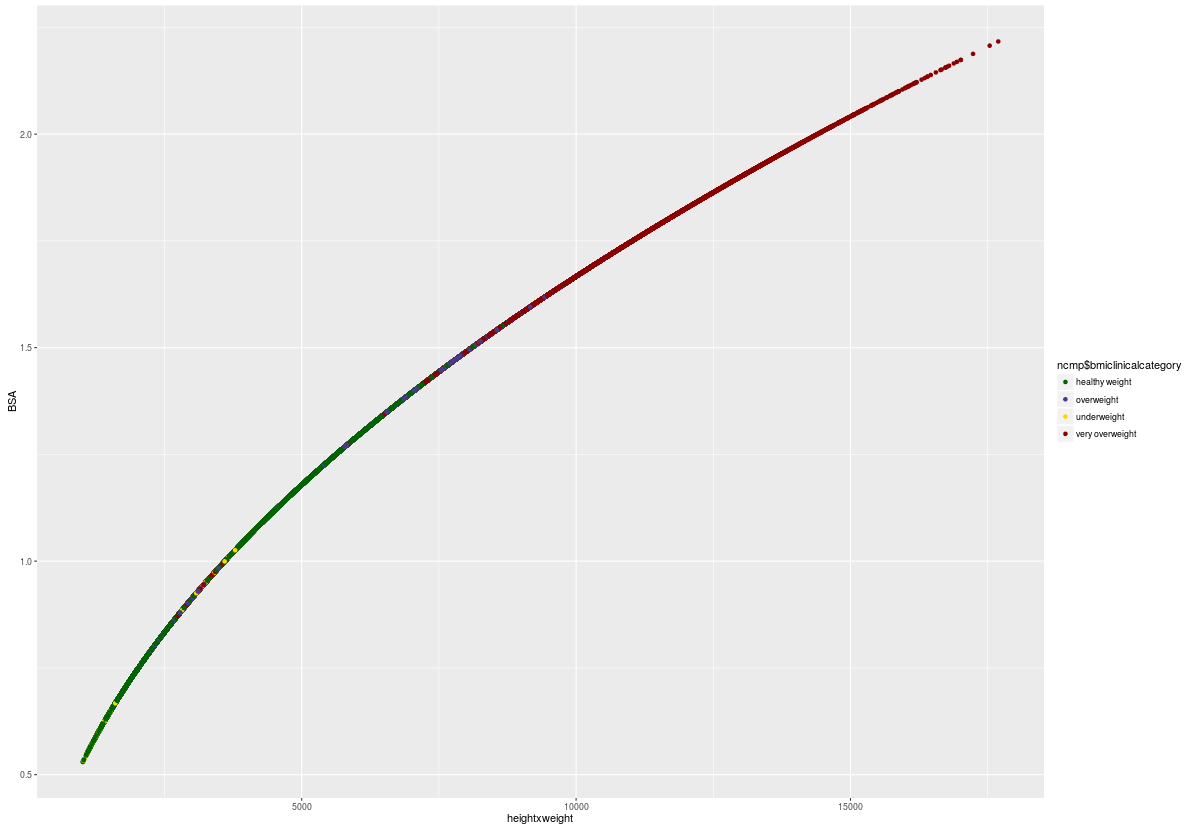
\includegraphics[scale=0.4]{xbsa.png}
			\end{center}
			\caption{Multiplication vs BSA}
		\end{figure}
<<<<<<< HEAD
In figure 9 we can see the relation between the body surface area and \(height\times weight\)
	\begin{figure}[H]
		\begin{center}
			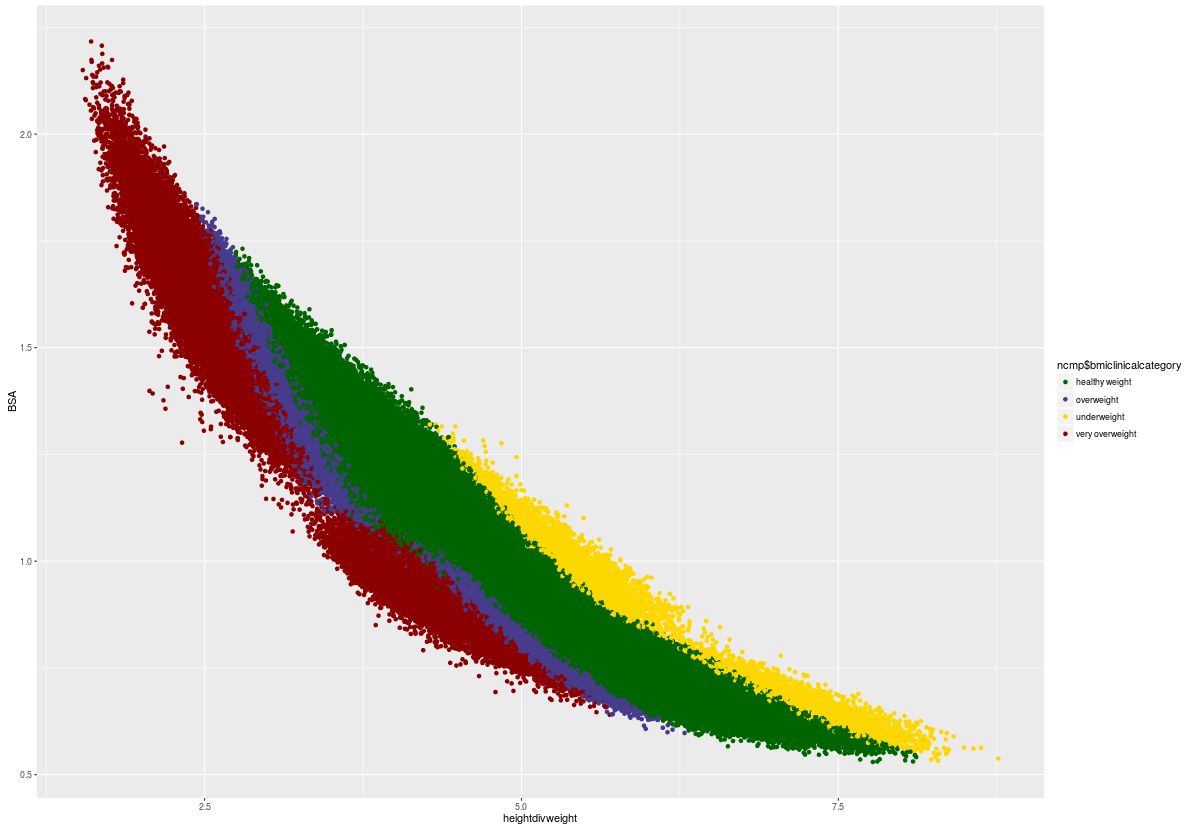
\includegraphics[scale=0.4]{divbsa.png}
		\end{center}
		\caption{Devision vs BSA}
	\end{figure}
	In figure 10 we can notice it's the inverse of figure 8 where the colors reversed and that's clearly because BMI category related to height and weight. So multiply them and divide them well give a contrast effect.
	\begin{figure}[H]
		\begin{center}
			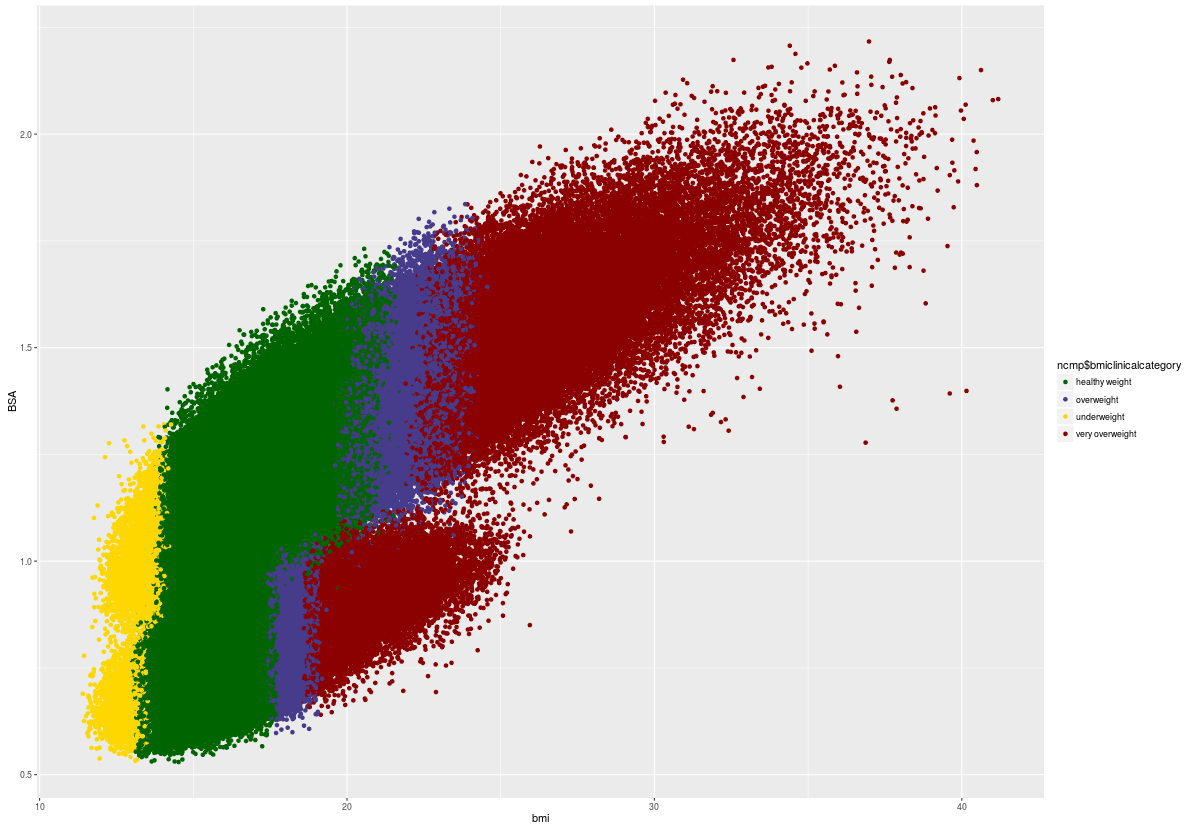
\includegraphics[scale=0.4]{bsabmi.png}
		\end{center}
		\caption{\textbf{BSA vs BMI}}
	\end{figure}
	In figure 11 we can see that BMI and BSA are correlated. And that's due how BSA \& BMI calculated.
\[BMI = \frac{Weight}{height^2}\]\[ , BSA = \frac{sqrt(height\times weight)}{60}\]
After that I calculated the correlation which was ~0.75
The previous figures and number generated by the following code :
\begin{lstlisting}[language=R]
######## Third Question ############
ncmp$heightxweight <- ncmp$height*ncmp$weight
ncmp$heightdivweight<-ncmp$height/ncmp$weight
ncmp$BSA<-sqrt(ncmp$heightxweight)/60

datasample$heightxweight <- datasample$height*datasample$weight
datasample$heightdivweight<-datasample$height/datasample$weight
datasample$BSA<-sqrt(datasample$heightxweight)/60

png ('xdiv.png',width = 1200,height = 830)
qplot(heightxweight,heightdivweight,data = ncmp,colour = ncmp$bmiclinicalcategory)+
scale_color_manual(values=c("darkgreen", "slateblue4","gold","darkred"))
dev.off()
png ('xbsa.png',width = 1200,height = 830)
qplot(heightxweight,BSA,data = ncmp,colour = ncmp$bmiclinicalcategory)+
scale_color_manual(values=c("darkgreen", "slateblue4","gold","darkred"))
dev.off()
png ('divbsa.png',width = 1200,height = 830)
qplot(heightdivweight,BSA,data = ncmp,colour = ncmp$bmiclinicalcategory)+
scale_color_manual(values=c("darkgreen", "slateblue4","gold","darkred"))
dev.off()
png ('bsabmi.png',width = 1200,height = 830)
qplot(bmi,BSA,data = ncmp,colour = ncmp$bmiclinicalcategory)+
scale_color_manual(values=c("darkgreen", "slateblue4","gold","darkred"))
dev.off()
cor(ncmp$BSA,ncmp$bmi)
\end{lstlisting}
Actually after noticing the formulas I thought about plotting density and here it: 
\begin{figure}[H]
\begin{center}
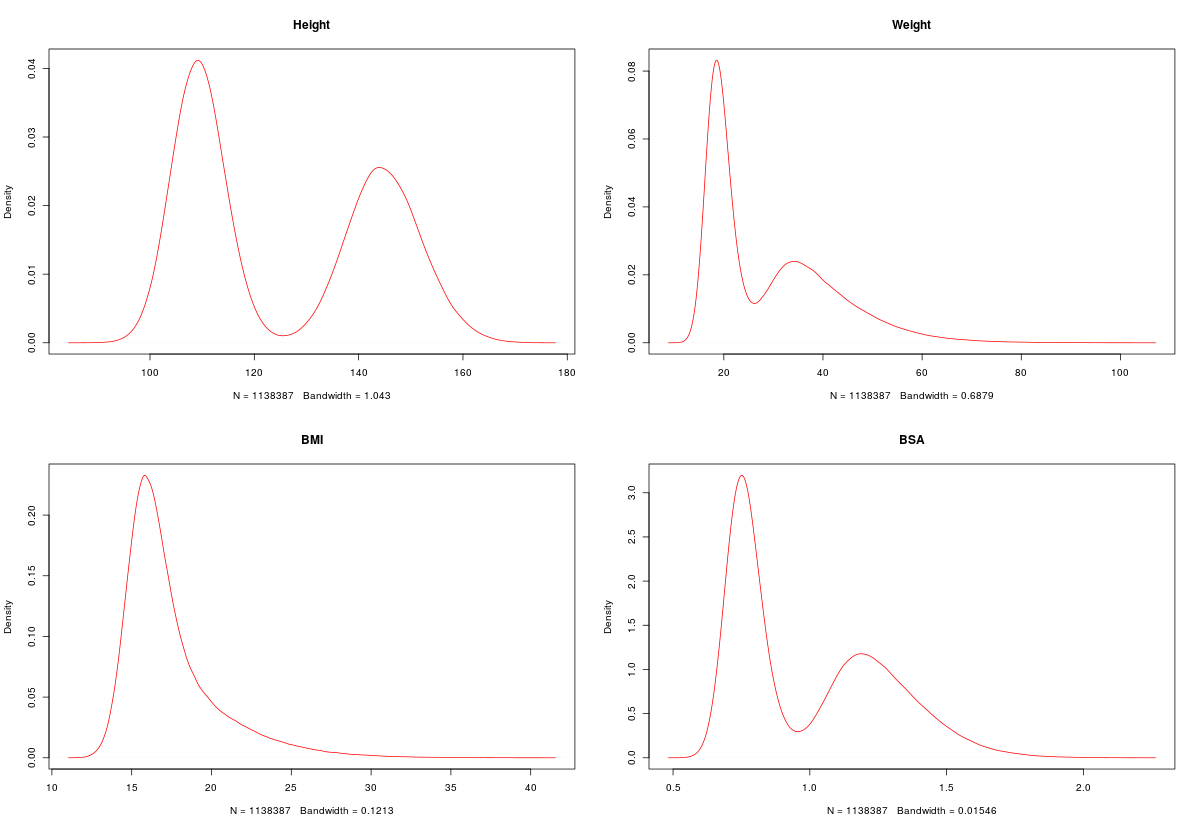
\includegraphics[scale=0.4]{density.png}
\end{center}
\caption{Density of Height,weight, BMI , BSA}
\end{figure}
Actually what we get from this is the reason of getting high BMI or BSA at specific time. maybe not the most useful one but I liked the idea :).
	\section*{Fourth Question}
	For this task I firstly created the groups.The gender group is clear but age group is not. There was two ways, one to use split and another to use what we analyzed in previous plots figures(4,5,7) where there is a break in age and show that we have two separated domains.
	In the next figure we can see the comparison between two plots before and after normalization 
\begin{figure}[H]
	\begin{center}
		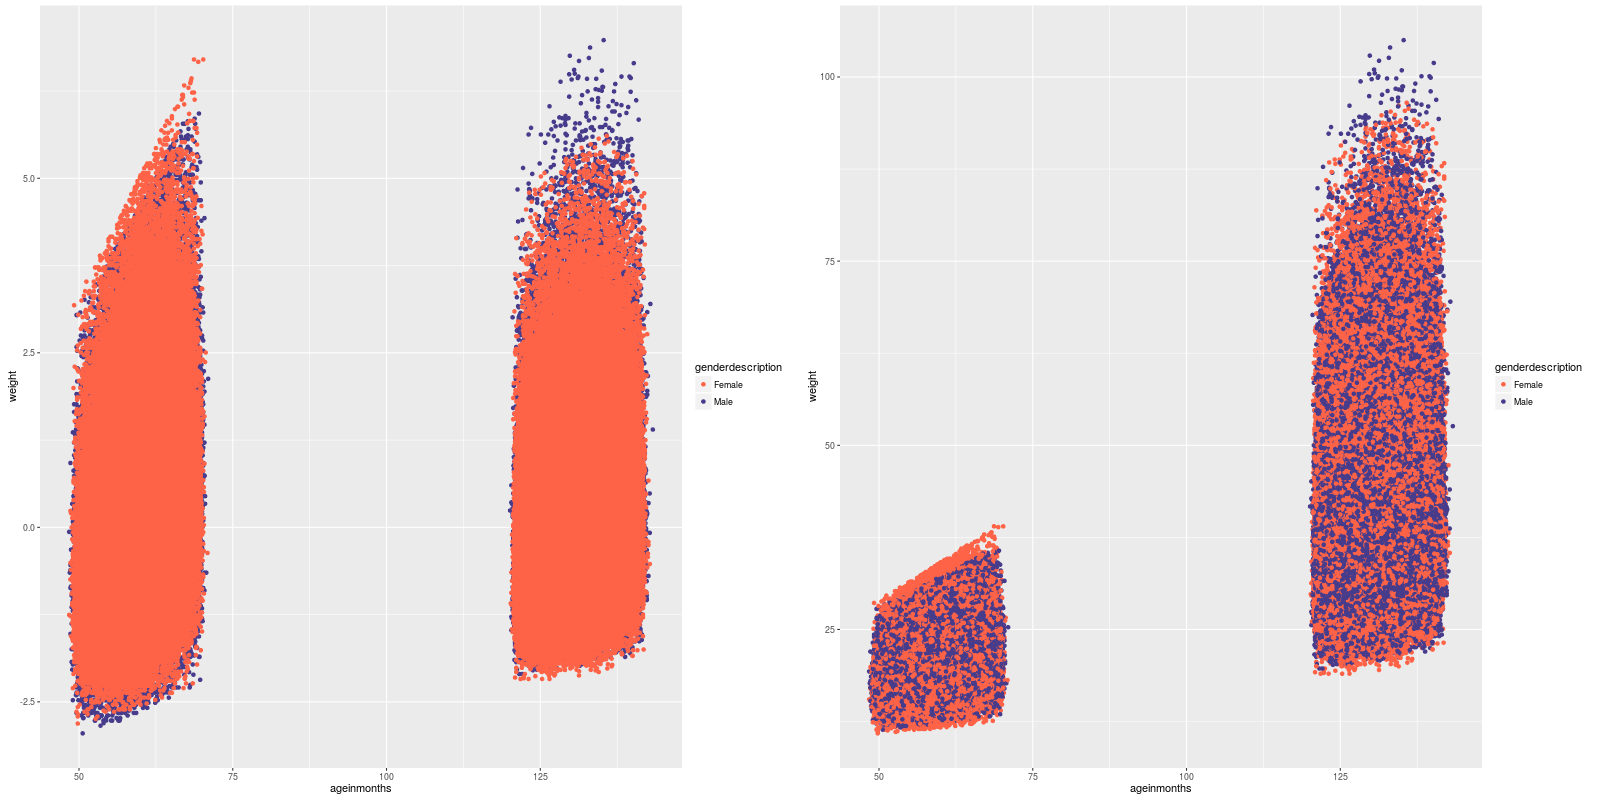
\includegraphics[scale=0.3]{normalizedageweightcomparsion.png}
	\end{center}
	\caption{Comparison before and after normalization}
\end{figure}
In figure 13 we can see that after normalization the density of dots are higher and the range is much less which give a clear prospective over the data.The problem is this type will increase the overlay of data (In case we want to distinguish 3rd dimension).
In figure 14 we can see Height vs weight after normalization it has the same problem as figure 13 of overlaying but we can draw conclusions about more height means more weight but not vise versa.
\begin{figure}[H]
	\begin{center}
		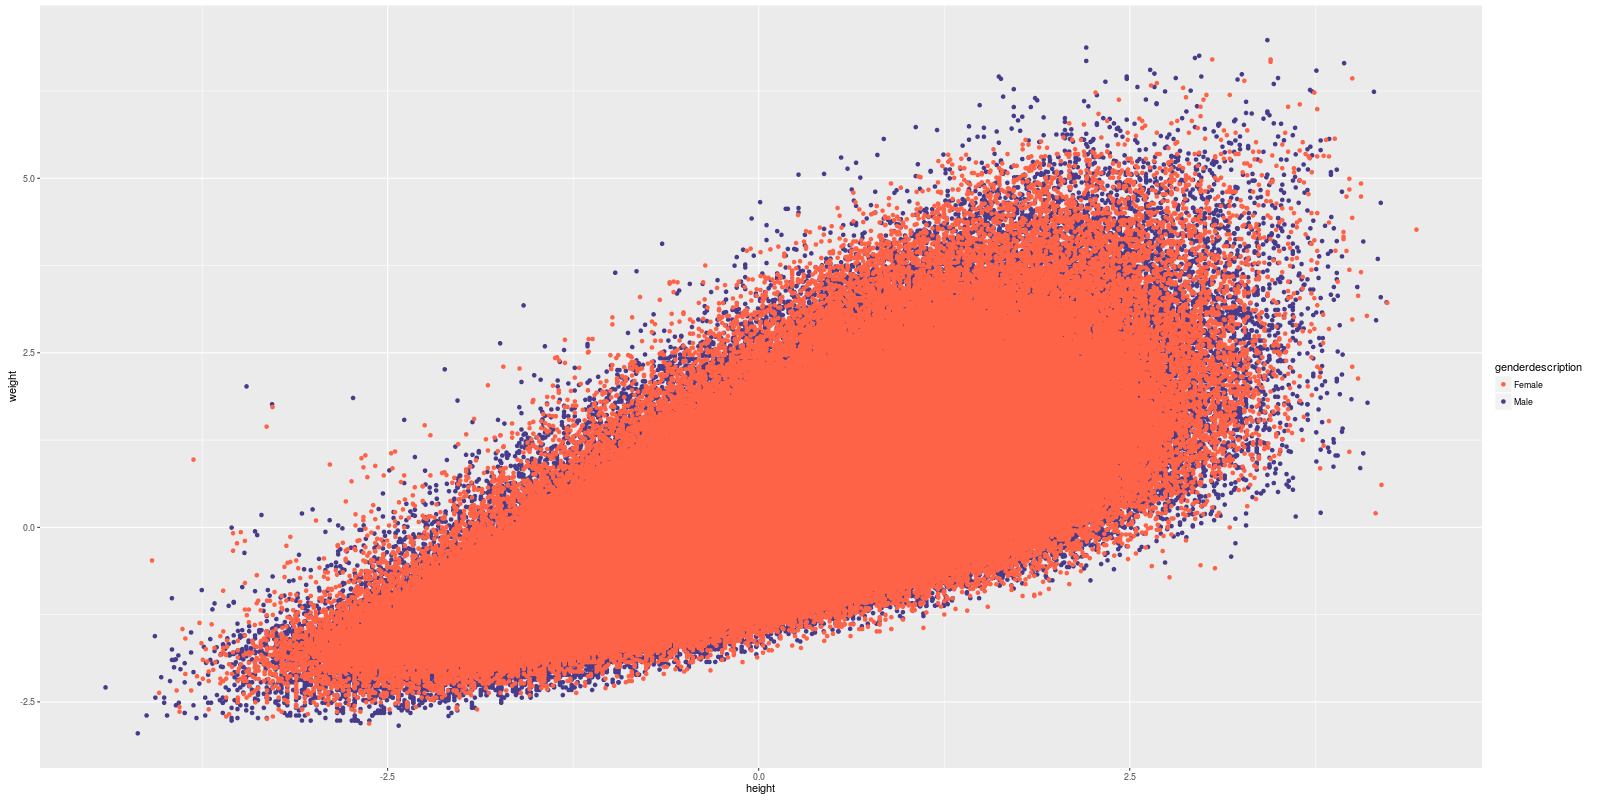
\includegraphics[scale=0.3]{heightweightnormalized.png}
	\end{center}
	\caption{Height vs weight after normalization}
\end{figure}

	I used function to show many ggplot library plots in same image. The function source is \href{http://www.cookbook-r.com/Graphs/Multiple_graphs_on_one_page_%28ggplot2%29/}{here} 
		here is the code for this function:
	\begin{lstlisting}[language=R]
# Multiple plot function
#
# ggplot objects can be passed in ..., or to plotlist (as a list of ggplot objects)
# - cols:   Number of columns in layout
# - layout: A matrix specifying the layout. If present, 'cols' is ignored.
#
# If the layout is something like matrix(c(1,2,3,3), nrow=2, byrow=TRUE),
# then plot 1 will go in the upper left, 2 will go in the upper right, and
# 3 will go all the way across the bottom.
#
multiplot <- function(..., plotlist=NULL, file, cols=1, layout=NULL) {
library(grid)

# Make a list from the ... arguments and plotlist
plots <- c(list(...), plotlist)

numPlots = length(plots)

# If layout is NULL, then use 'cols' to determine layout
if (is.null(layout)) {
# Make the panel
# ncol: Number of columns of plots
# nrow: Number of rows needed, calculated from # of cols
layout <- matrix(seq(1, cols * ceiling(numPlots/cols)),
ncol = cols, nrow = ceiling(numPlots/cols))
}

if (numPlots==1) {
print(plots[[1]])

} else {
# Set up the page
grid.newpage()
pushViewport(viewport(layout = grid.layout(nrow(layout), ncol(layout))))

# Make each plot, in the correct location
for (i in 1:numPlots) {
# Get the i,j matrix positions of the regions that contain this subplot
matchidx <- as.data.frame(which(layout == i, arr.ind = TRUE))

print(plots[[i]], vp = viewport(layout.pos.row = matchidx$row,
layout.pos.col = matchidx$col))
}
}
}
	\end{lstlisting}
For normalization I used this formula \(X_n = \frac{X-\mu}{\sigma}\) to normalize the weight and height.
	The code for this task : 
	\begin{lstlisting}[language=R]
###### Fourth Question ######
normalize<-function(x)
{
return ((x-mean(x))/sd(x))
}
maleunder100<-ncmp[ncmp$genderdescription=='Male'&ncmp$ageinmonth<100,]
maleunder100$height<- normalize(maleunder100$height)
maleunder100$weight<- normalize(maleunder100$weight)
maleabove100<-ncmp[ncmp$genderdescription=='Male'&ncmp$ageinmonth>100,]
maleabove100$height<- normalize(maleabove100$height)
maleabove100$weight<- normalize(maleabove100$weight)
femaleunder100<-ncmp[ncmp$genderdescription=='Female'&ncmp$ageinmonth<100,]
femaleunder100$height<- normalize(femaleunder100$height)
femaleunder100$weight<- normalize(femaleunder100$weight)
femaleabove100<-ncmp[ncmp$genderdescription=='Female'&ncmp$ageinmonth>100,]
femaleabove100$height<- normalize(femaleabove100$height)
femaleabove100$weight<- normalize(femaleabove100$weight)
normalizedncmp<-rbind(maleunder100,maleabove100,femaleunder100,femaleabove100)
##Another Way to do previous split
#gs<- split(ncmp,datasample$genderdescription)

#age,weight normalized
png('normalizedageweightcomparsion',height = 800,width = 1600)
p1<-qplot(ageinmonths,weight,colour =genderdescription,data = normalizedncmp)+ 
scale_color_manual(values=c("tomato", "slateblue4"))
# age weight
p2<-qplot(ageinmonths,weight,colour =genderdescription,data = ncmp)+ 
scale_color_manual(values=c("tomato", "slateblue4"))
multiplot(p1,p2,cols = 2)
dev.off()
# BMI weight
png('BMIweightnormalied.png',height = 800,width = 1600)
qplot(bmi,weight,colour =genderdescription,data = normalizedncmp)+ 
scale_color_manual(values=c("tomato", "slateblue4"))
dev.off()

#Height Weight
png('heightweightnormalized.png',height = 800,width = 1600)
qplot(height,weight,colour =genderdescription,data = normalizedncmp)+ 
scale_color_manual(values=c("tomato", "slateblue4"))
dev.off()
	\end{lstlisting}
	\section*{Fifth Question}
In this question first I created a function to separate data into quantiles and then aggregate them.
I divided the data depending on age into two groups from [49.1,70.0] and [120.8,141.4] and that's to prevent the break between them from shown.\\
The data also separated depending on gender as requested in the question.Here is the figures
\begin{figure}[H]
\begin{center}
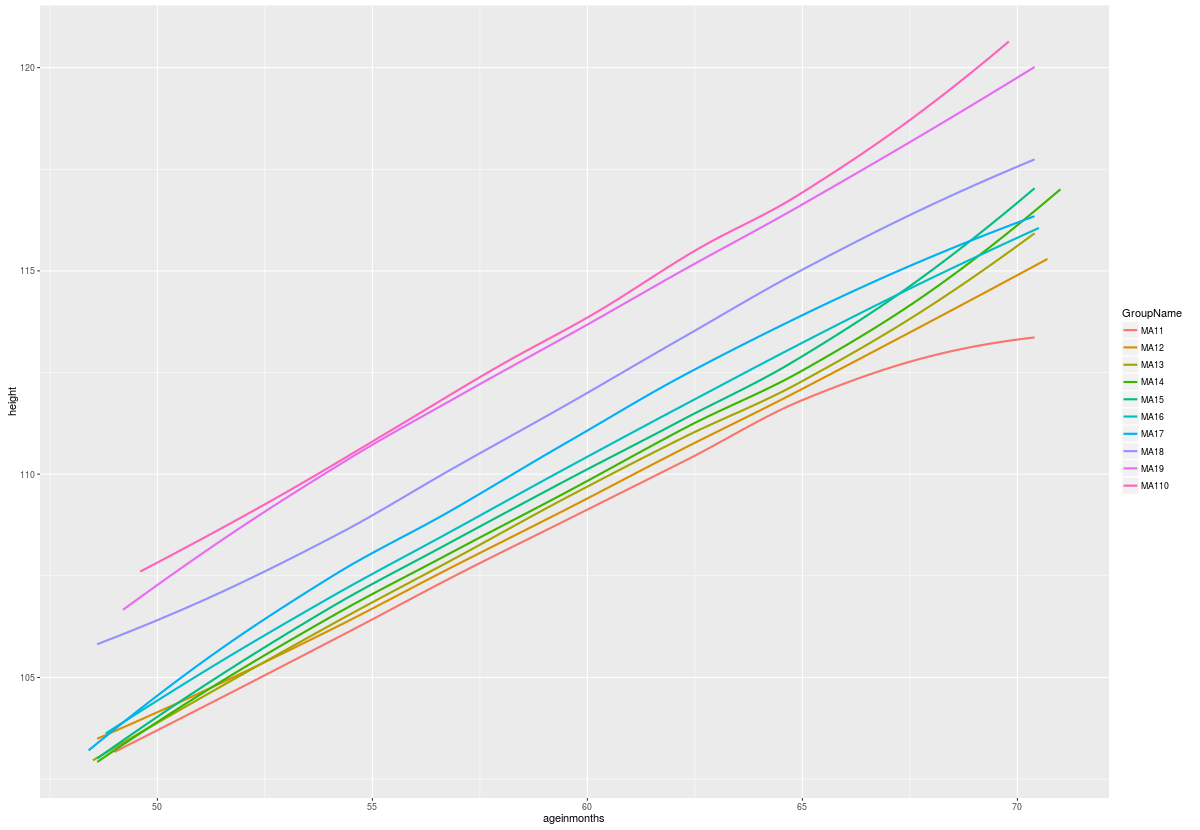
\includegraphics[scale = 0.4]{maleage1.png}
\end{center}
\caption{Males in age area 1 vs height}
\end{figure} 
In the previous figure MA11 mean Male Age 1(Area 1) ,1(1st Quantile of BMI).
\begin{figure}[H]
	\begin{center}
		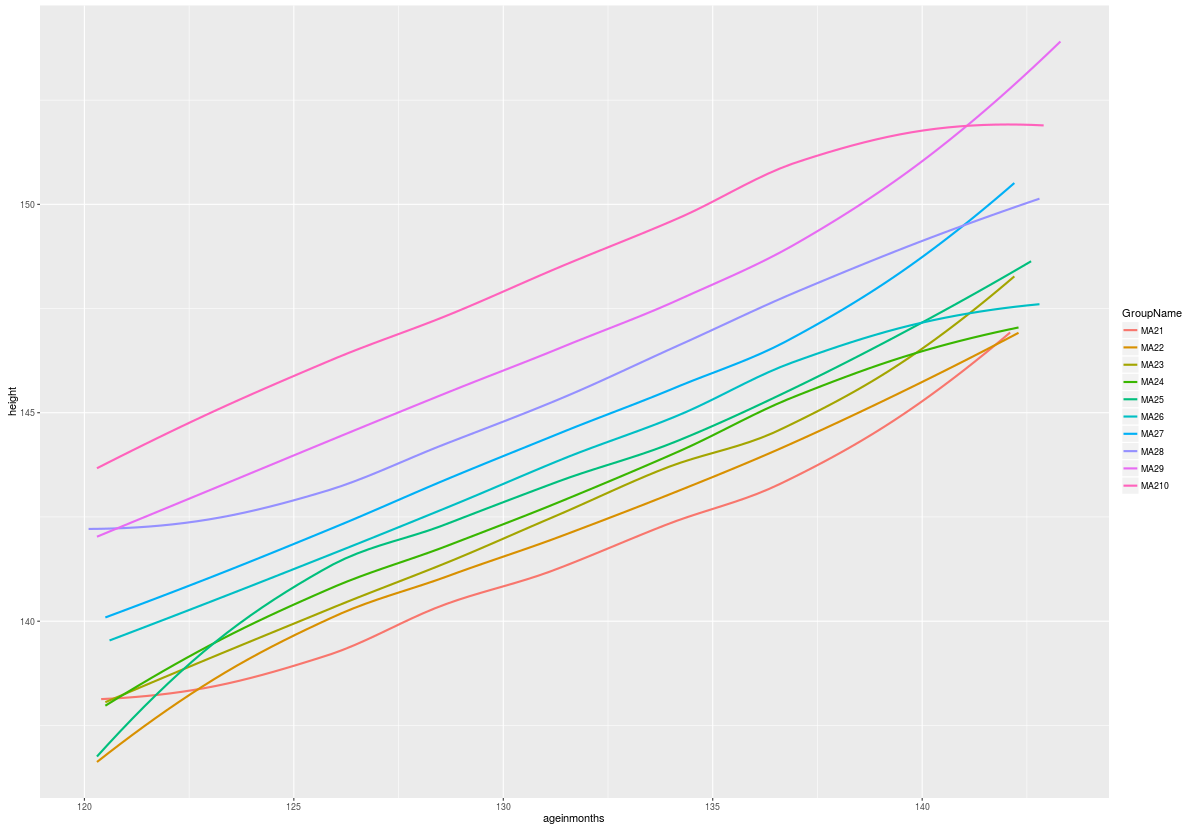
\includegraphics[scale = 0.4]{maleage2.png}
	\end{center}
	\caption{Males in age area 2 vs height}
\end{figure} 

\begin{figure}[H]
	\begin{center}
		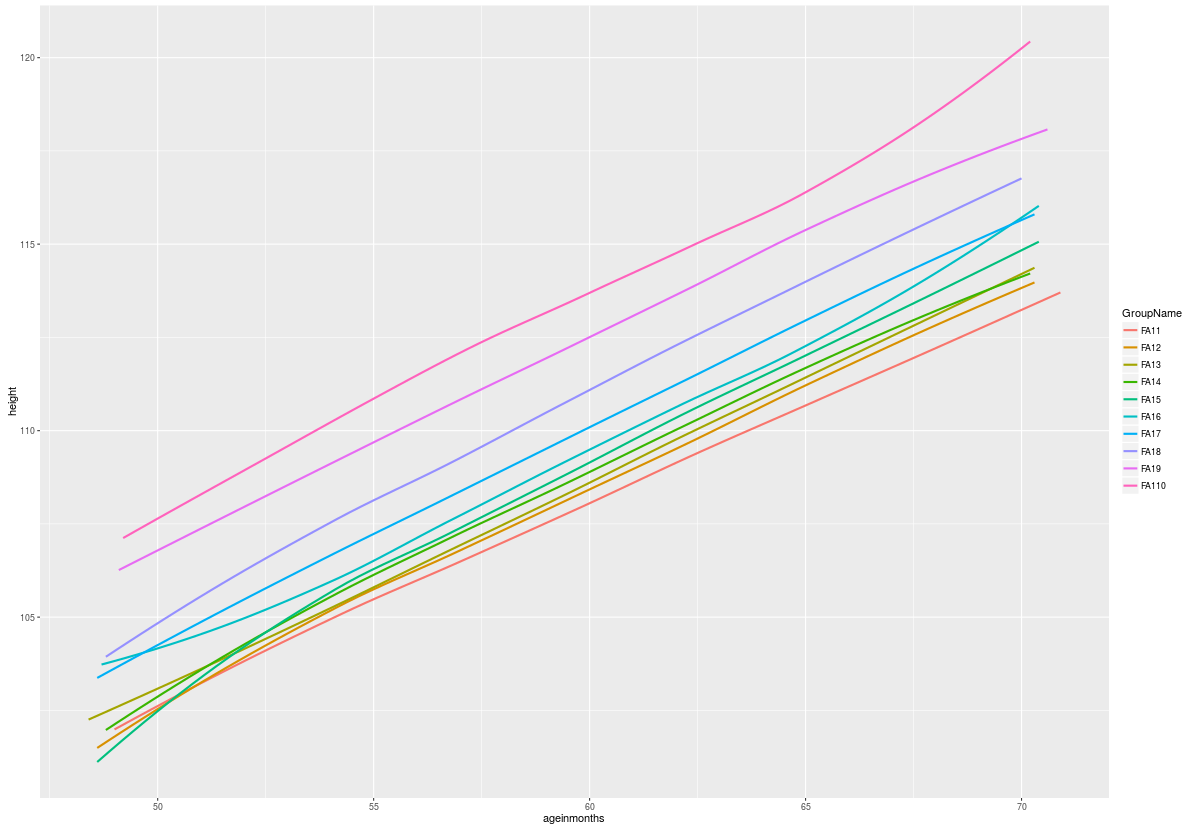
\includegraphics[scale = 0.4]{femaleage1.png}
	\end{center}
	\caption{Females in age area 1 vs height}
\end{figure}

\begin{figure}[H]
	\begin{center}
		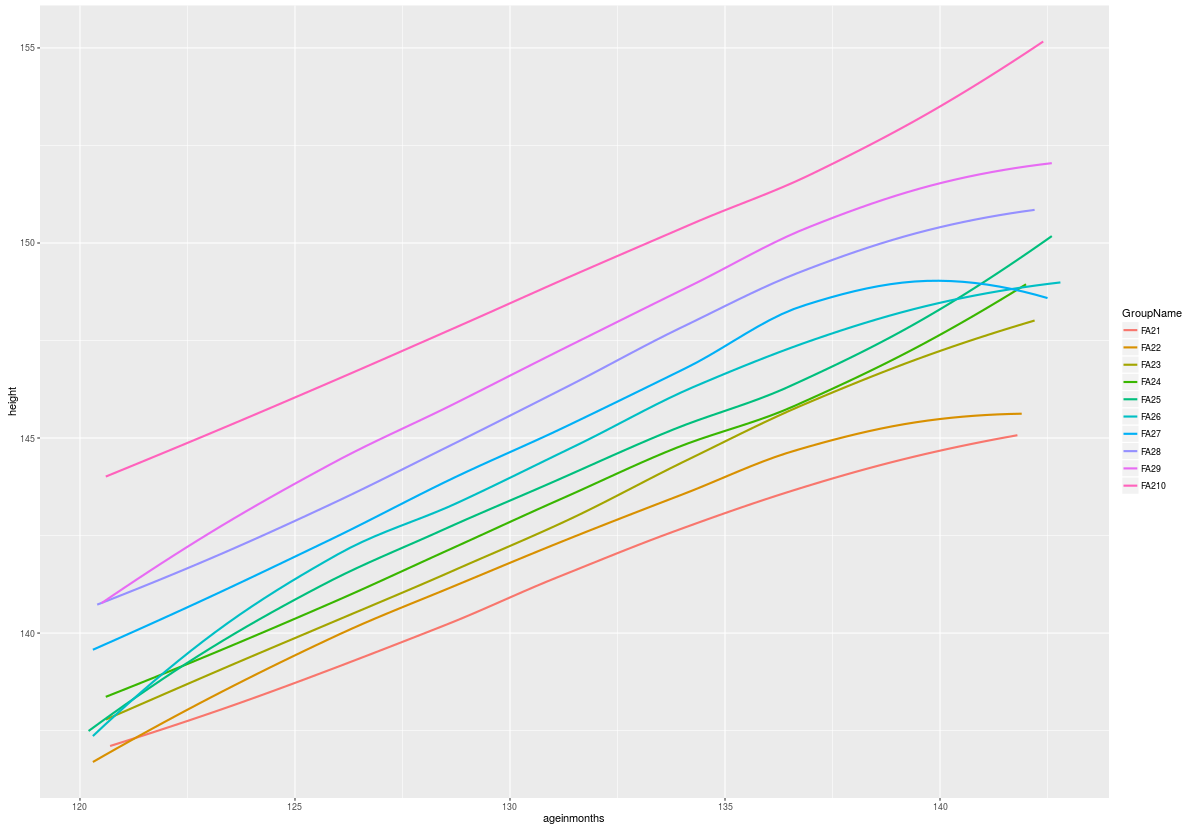
\includegraphics[scale = 0.4]{femaleage2.png}
	\end{center}
	\caption{Females in age area 2 vs height}
\end{figure}  

The generated figures and the functions and the code is here:
\begin{lstlisting}[language=R]
########## Fifth Question ##############
#Function return data in quantiles
CreateQuantiles<-function(x,groupname)
{
#Create Qunatiles
qu <-quantile(datasample$bmi,probs = seq(0,1,0.1))
qu.list<-list()
for (i in seq(1,10,1))
{
qu.list[[i]]<-x[x$bmi>qu[i] & x$bmi<qu[i+1],]

}
result<-data.frame()
#Create Aggregation
for (i in seq(1,10,1))
{
qu.list[[i]]<-aggregate(height ~ ageinmonths,qu.list[[i]], mean)
GroupName=paste(groupname,toString(i),sep = '')
result<-rbind(result,cbind(qu.list[[i]],GroupName))
}
return(result)
}
agelimits<-c(48,72.0,120,144)
sort(unique(ncmp$ageinmonths))
maleage1 <-CreateQuantiles(ncmp[ncmp$ageinmonths>agelimits[1] & ncmp$ageinmonths<agelimits[2]&
ncmp$genderdescription=="Male",],'MA1')
png ('maleage1.png',width = 1200,height = 830)
ggplot(data=maleage1, aes(x=ageinmonths, y=height, group = GroupName, colour = GroupName)) +
geom_smooth(se = FALSE)
dev.off()
maleage2 <-CreateQuantiles(ncmp[ncmp$ageinmonths>agelimits[3] & ncmp$ageinmonths<agelimits[4]&
ncmp$genderdescription=="Male",],'MA2')
png ('maleage2.png',width = 1200,height = 830)
ggplot(data=maleage2, aes(x=ageinmonths, y=height, group = GroupName, colour = GroupName)) +
geom_smooth(se = FALSE)
dev.off()
femaleage1 <-CreateQuantiles(ncmp[ncmp$ageinmonths>agelimits[1] & ncmp$ageinmonths<agelimits[2]&
ncmp$genderdescription=="Female",],'FA1')
png ('femaleage1.png',width = 1200,height = 830)
ggplot(data=femaleage1, aes(x=ageinmonths, y=height, group = GroupName, colour = GroupName)) +
geom_smooth(se = FALSE)
dev.off()
femaleage2 <-CreateQuantiles(ncmp[ncmp$ageinmonths>agelimits[3] & ncmp$ageinmonths<agelimits[4]&
ncmp$genderdescription=="Female",],'FA2')
png ('femaleage2.png',width = 1200,height = 830)
ggplot(data=femaleage2, aes(x=ageinmonths, y=height, group = GroupName, colour = GroupName)) +
geom_smooth(se = FALSE)
dev.off()
\end{lstlisting}
	\section*{Sixth Question}
There were many projects. The ones I remeber better are : 
\begin{enumerate}
\item \textbf{Kindergarden/Schools Planing:} as I recall it was about managing placing kids in schools and kinder gardens. Help in relocating (maybe about creating schools and stuff like that can't recall accurately :( ))
\item \textbf{City Data/Infratructure:} Was about creating a map of the city with information about age of buildings to imagine how the city created.
\item \textbf{Public Taxis/Urban Biodevice city/Public Space planing} (recall merging all those)  It was about providing a better city planing for stops can't recall much:( 
\end{enumerate} 
 my selection was on Crime/Danger / Violent which is not mention in previous list because the full report is below.\\

\subsection*{\Large Crime / Danger / Violent}
\textbf{\large What Data?}
\begin{enumerate}
\item		Accidents.
\item		Location of crime from police.
\item		Crimes (street crimes, bribes).
\item 		Tax paying violations.
\item		Fights.
\item		Drug usage.
\item		Slippery roads.
\item		Wrong parking.
\item		Shop lifting.
\item		Rescue services data from events
\end{enumerate}
\textbf{\large Data Description?}\\
	\(|\) Date \(|\)  location\(|\)  time\(|\)  people involved\(|\)  people injured \(|\)  type of crime\(|\)  event description \(|\) what was stolen\(|\)  type of injure\(|\)  gender\(|\)  \\
	NOTE: Gather information also from crowd-source platforms.\\
	\textbf{\large Why?}
	\begin{enumerate}
\item			Assess possible risks from the data by regular people
\item			Get better overview for handling crimes for Police
\item			Rebuild streets and add zebras / signs / street lighting
\item			To determine crime rate and to predict the security need for shops
\item			To estimate real estate value with actual visible data
	\end{enumerate}

	\textbf{\large Service / Prototype?}	
	\begin{enumerate}
\item	48 – Hours: build a website and App
\item	Crime report APP (Co-ordinates, nature of crime)
\item	To predict future location / future crimes
\item	To visualize current crime levels
	\end{enumerate}

\textbf{\Large Note:} All the code,images,report,latex for this home work exist in \href{https://github.com/aqeel13932/DM/tree/master/HW04}{this github channel}
=======
				\begin{figure}[H]
					\begin{center}
						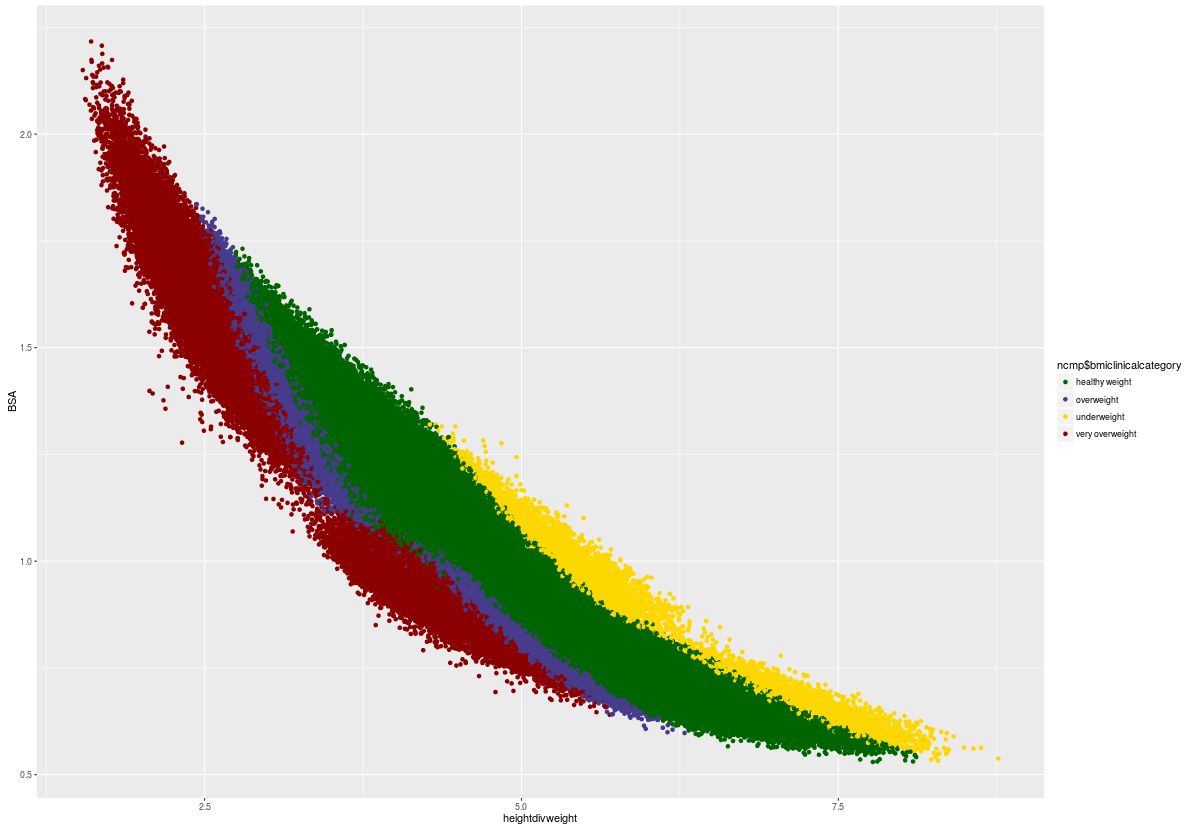
\includegraphics[scale=0.4]{divbsa.png}
					\end{center}
					\caption{Devision vs BSA}
				\end{figure}
	\section*{Fourth Question}
	\section*{Fifth Question}
	\section*{Sixth Question}
>>>>>>> 59314da8caff27eef4431dda7d1964df874949c5
\end{document}